\section(Aircraft ground handling and human factors [Hey, you just read this, and you are thinking, not a gu'd headline, so change it maybe?])
In NLR Air Transport Safety Institutes [insert relation to European Commercial Aviation Safety Team] report, \"Aircraft ground handling and human factors\" finished in April 2010, on the; \"... causal factors which lead to human errors during the ground handling process and create unsafe situations, personal accidents or incidents.\" (Page 1 of the report) found that the largest safety related issues in operational personnel and management comes from \"standardisation of phraseology on the ramp\" and human factors such as time pressure, stress, fatigue and communication. This part of the report will describe the detailed findings of the [undersøgelse?] related to this project and their recommendations to the ground handling companies.

First of all one of the interesting findings was that of which the frequency of incidents happens and in which categories they happens. In figure \ref{FrequencyOfIncidents} we can clearly see that both incidents that cause operational disruptions, equipment damage and aircraft damage each happens at least once a weak. As decried in section [Freight] not only will damage be costly to repair it also most likely causes airplane delays which can be very expesive for th airlines. Of cause operational discrupts also results in delays
\begin{figure}
\centering
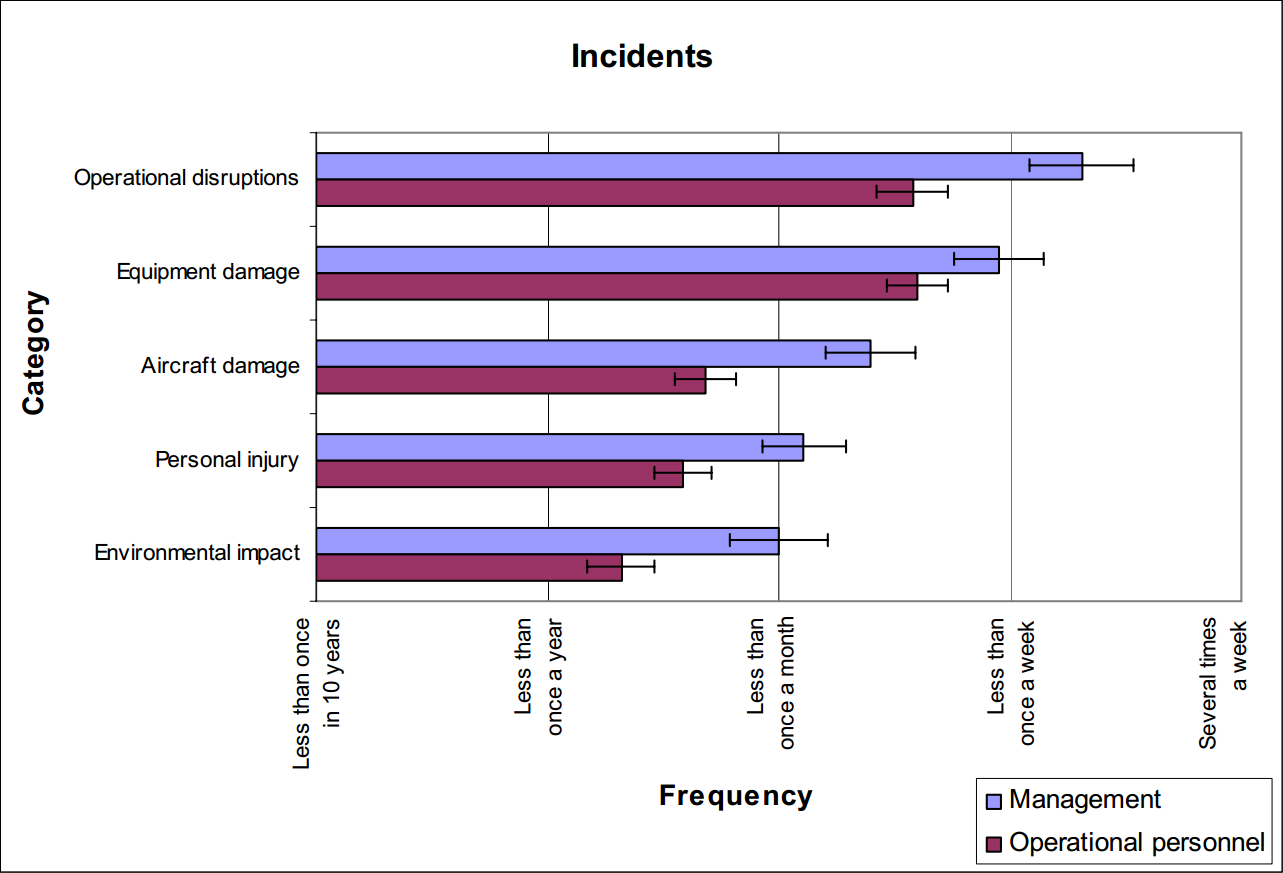
\includegraphics{Grafik/FrequencyOfIncidents}
\caption{The frequency of how often incidents of different categories happens.}
\label{FrequencyOfIncidents}
\end{figure}

(You got to page 29)

\begin{figure}
\centering
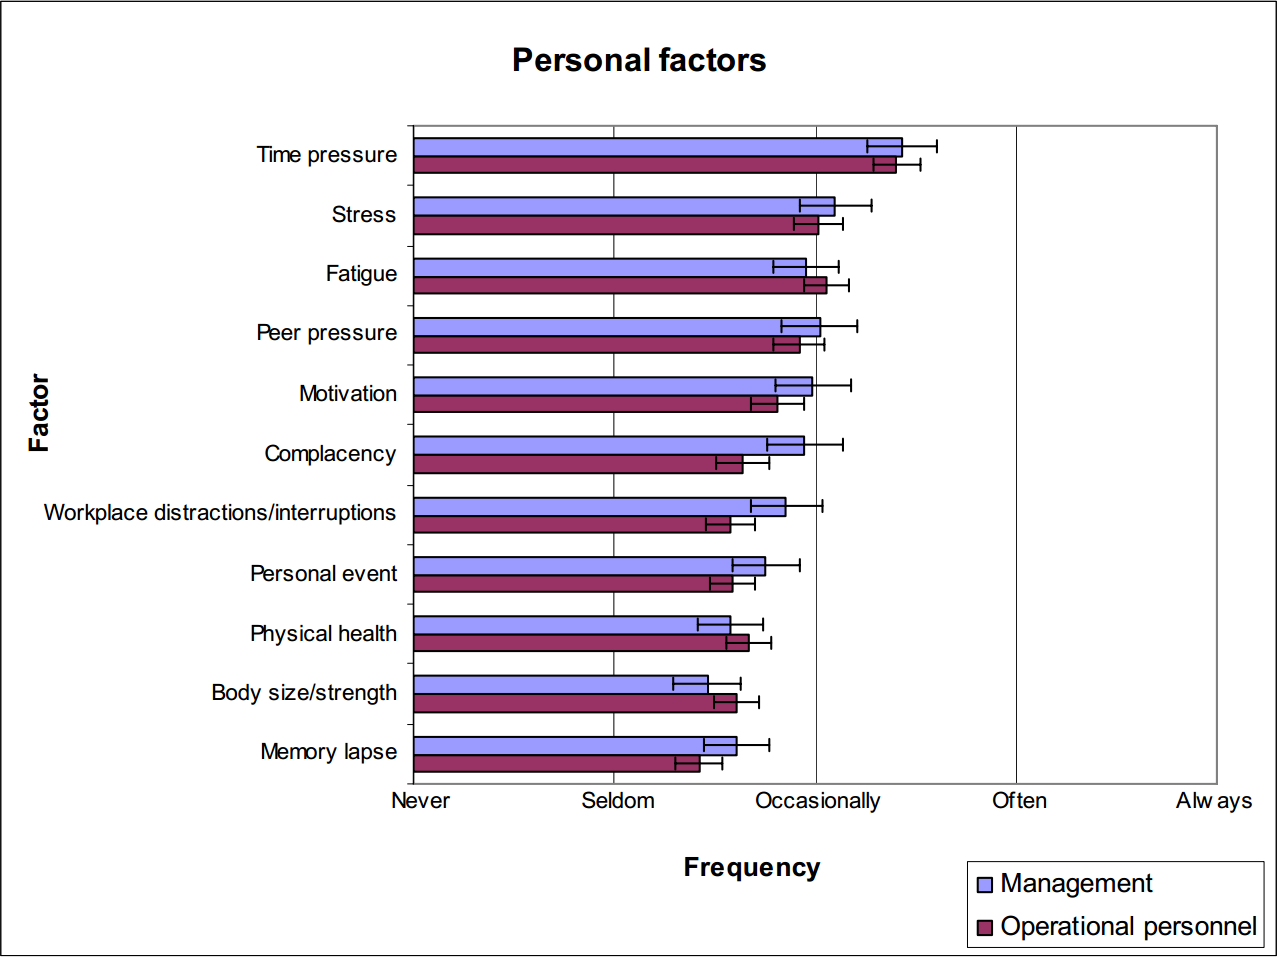
\includegraphics{Grafik/PersonalFactors}
\caption{Breakdown of channels used to book flights.}
\label{PersonalFactors}
\end{figure}